% Native editable composition from verified, unchanged IDE images.
\par
\begin{figure}[htbp]
  \centering
  \sbox0{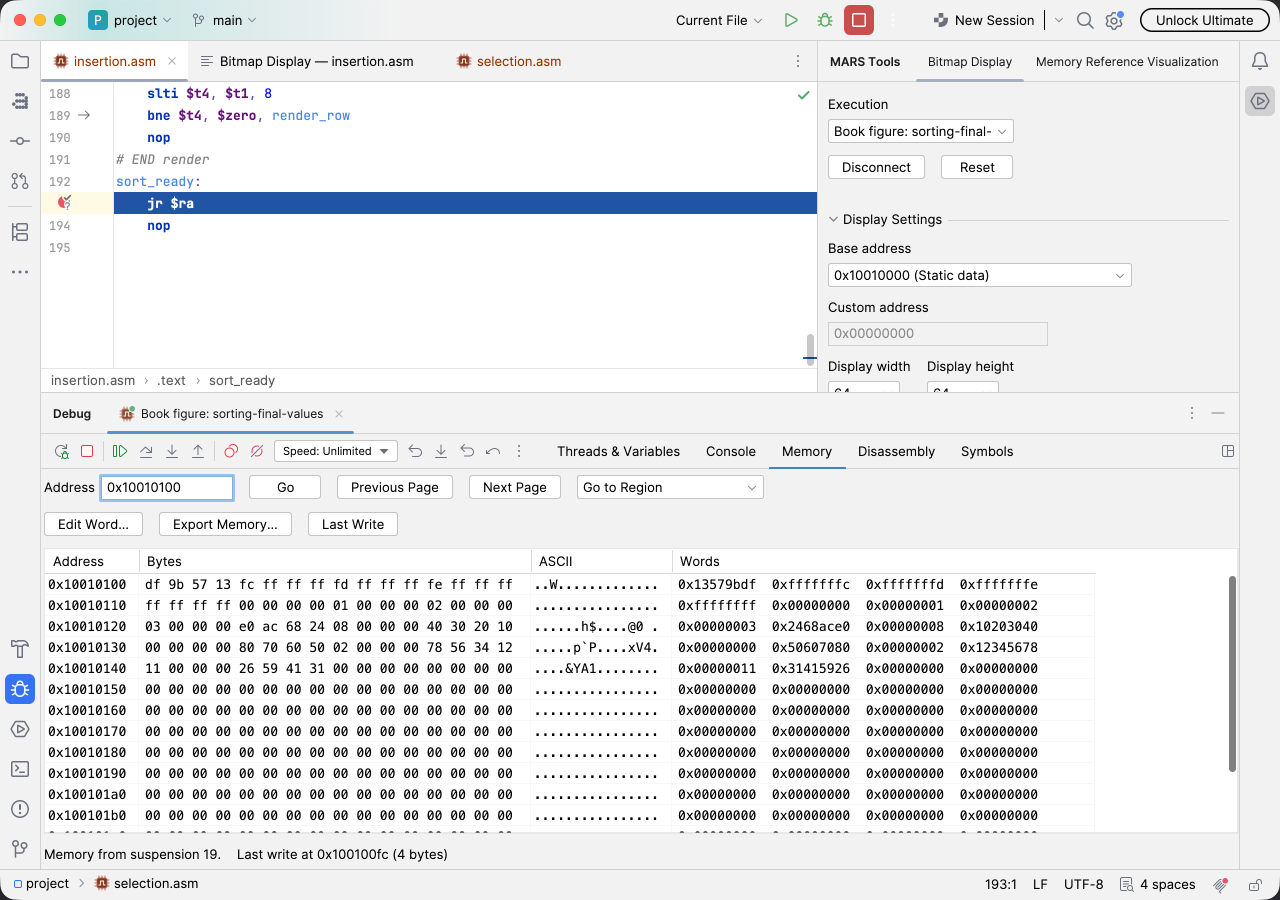
\includegraphics[artifact]{packages/009-sorting-visualizer/captures/f04-final/values.png}}
  \sbox2{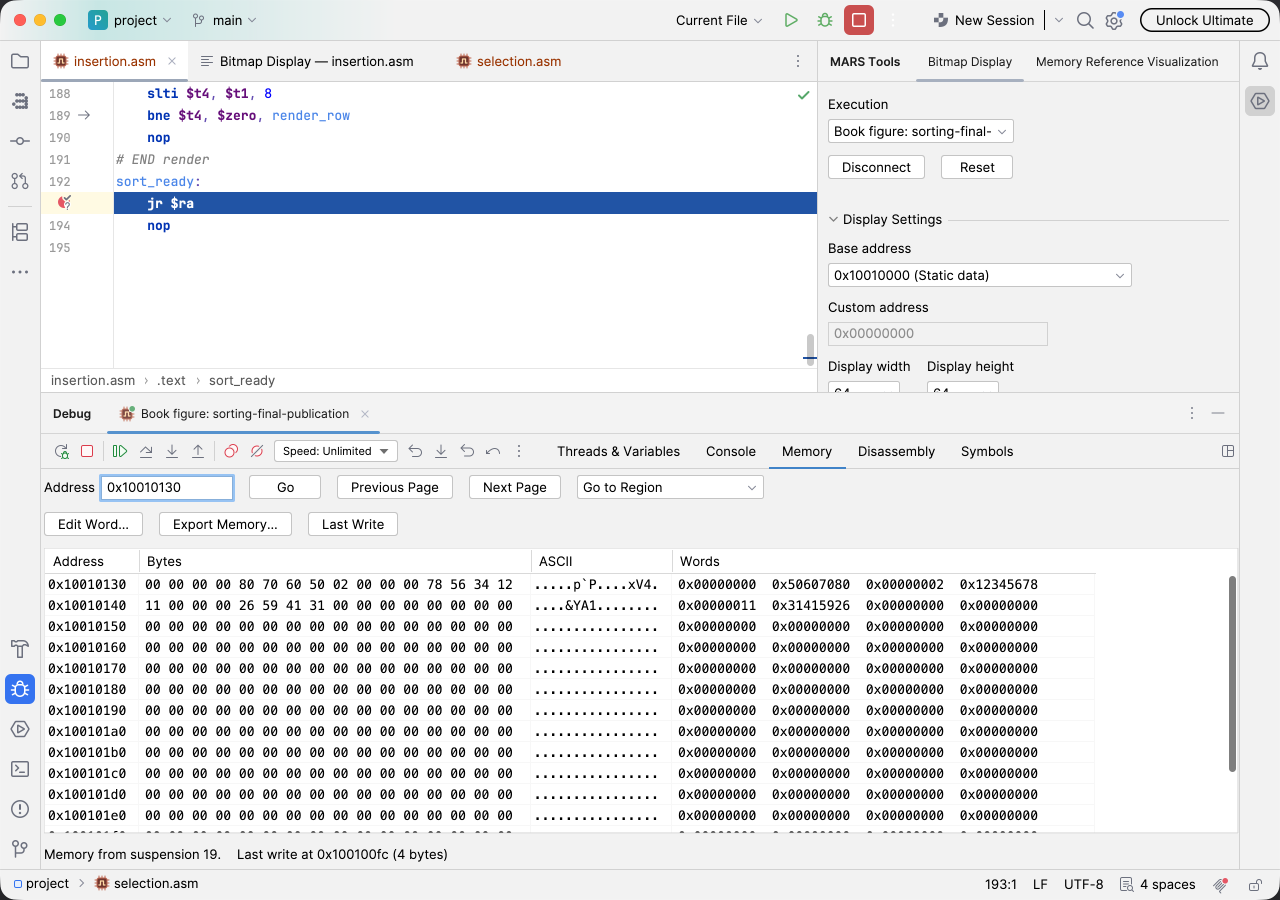
\includegraphics[artifact]{packages/009-sorting-visualizer/captures/f04-final/publication.png}}
  \sbox4{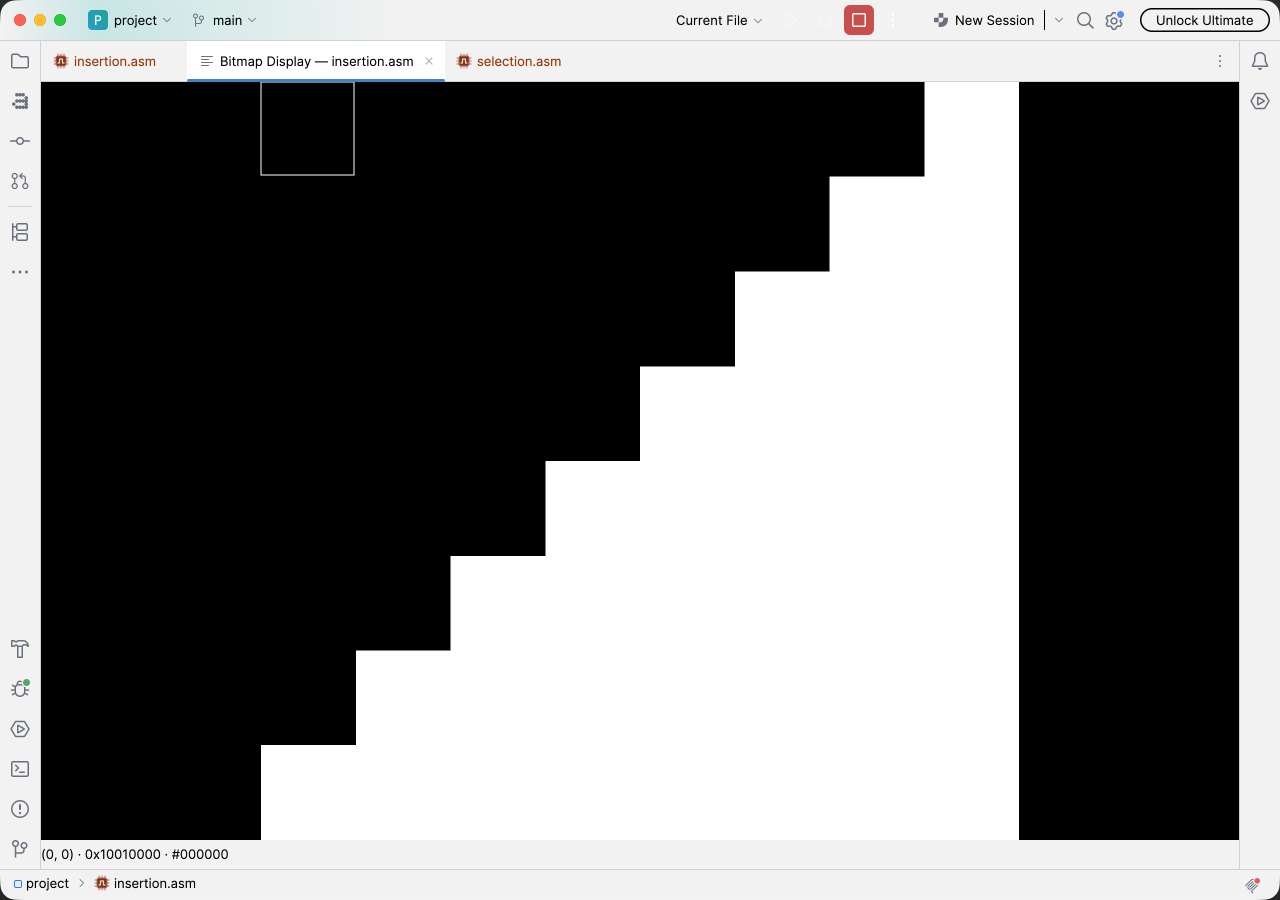
\includegraphics[artifact]{packages/009-sorting-visualizer/captures/f04-final/bitmap.png}}
  \edef\MARSfinalsourceLeft{\the\dimexpr0.036718750\wd0\relax}
  \edef\MARSfinalsourceBottom{\the\dimexpr0.757777778\ht0\relax}
  \edef\MARSfinalsourceRight{\the\dimexpr0.611718750\wd0\relax}
  \edef\MARSfinalsourceTop{\the\dimexpr0.164444444\ht0\relax}
  \edef\MARSfinalstateLeft{\the\dimexpr0.034375000\wd0\relax}
  \edef\MARSfinalstateBottom{\the\dimexpr0.287777778\ht0\relax}
  \edef\MARSfinalstateRight{\the\dimexpr0.578906250\wd0\relax}
  \edef\MARSfinalstateTop{\the\dimexpr0.608888889\ht0\relax}
  \edef\MARSfinalmemoryLeft{\the\dimexpr0.034375000\wd2\relax}
  \edef\MARSfinalmemoryBottom{\the\dimexpr0.311111111\ht2\relax}
  \edef\MARSfinalmemoryRight{\the\dimexpr0.578906250\wd2\relax}
  \edef\MARSfinalmemoryTop{\the\dimexpr0.608888889\ht2\relax}
  \edef\MARSfinalplotLeft{\the\dimexpr0.203906250\wd4\relax}
  \edef\MARSfinalplotBottom{\the\dimexpr0.066666667\ht4\relax}
  \edef\MARSfinalplotRight{\the\dimexpr0.203906250\wd4\relax}
  \edef\MARSfinalplotTop{\the\dimexpr0.091111111\ht4\relax}
  \begin{tikzpicture}[alt={Four annotated details at insertion completion before the renderer returns. Values are minus four, minus three, minus two, minus one, zero, one, two, three. Selector is zero, phase is two and the exchange count is decimal seventeen, stored as hexadecimal eleven. White bar heights rise from one through eight.}]
    \node[anchor=north west,inner sep=0,font=\small\bfseries] (source-title) at (6mm,0) {Next instruction: return from the renderer};
    \node[anchor=north west,inner sep=0] (source) at ([yshift=-1mm]source-title.south west) {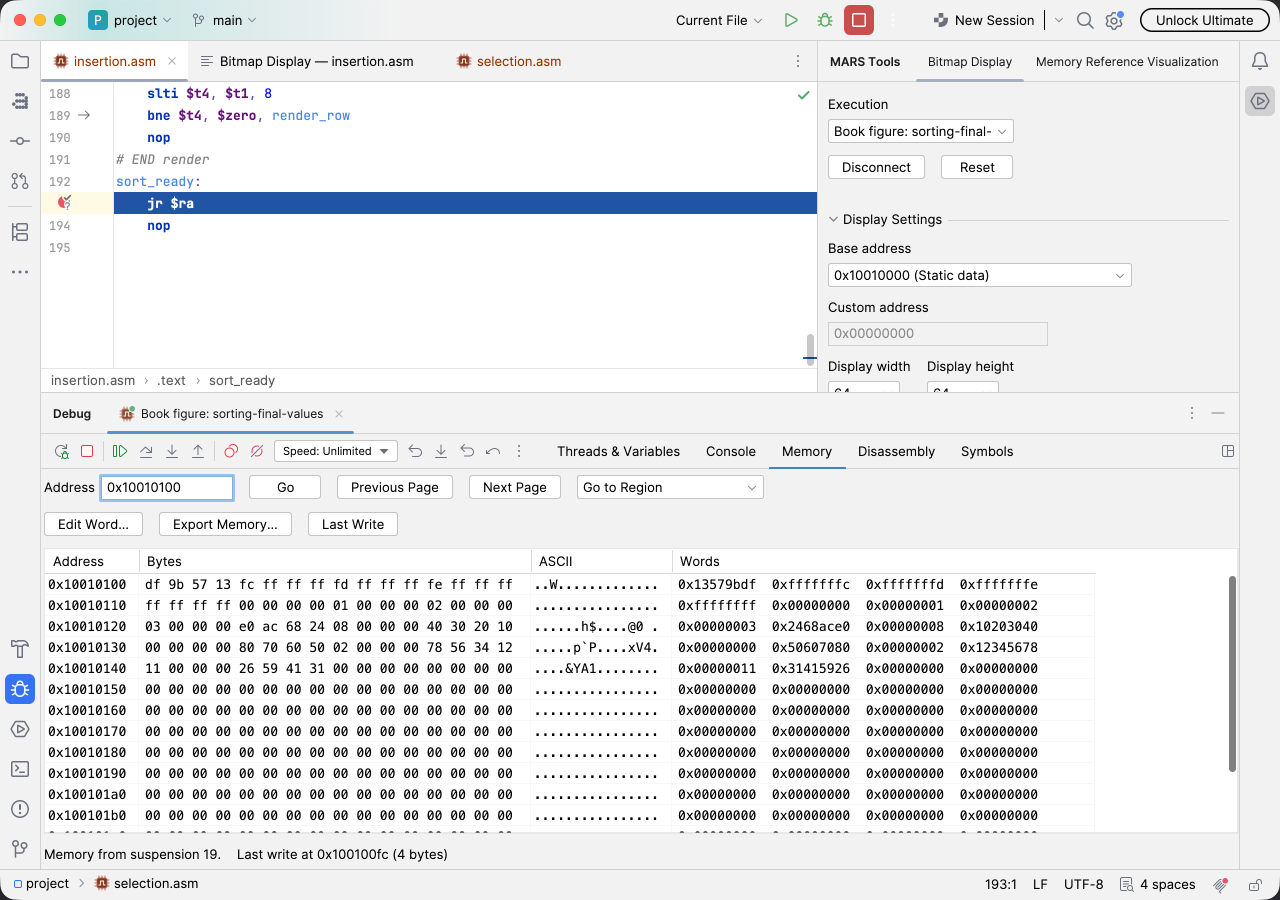
\includegraphics[width=0.7\linewidth,artifact,trim={\MARSfinalsourceLeft{} \MARSfinalsourceBottom{} \MARSfinalsourceRight{} \MARSfinalsourceTop{}},clip]{packages/009-sorting-visualizer/captures/f04-final/values.png}};
    \begin{scope}[shift={(source.south west)},x={($(source.south east)-(source.south west)$)},y={($(source.north west)-(source.south west)$)}]
      \draw[black,line width=0.7pt] (0.153333333,0.057142857) rectangle (0.326666667,0.371428571);
      \node[draw=black,fill=white,circle,inner sep=1.5pt,font=\footnotesize] at ($(0.153333333,0.371428571)+(-3mm,0)$) {1};
    \end{scope}
    \node[anchor=north west,inner sep=0,font=\small\bfseries] (state-title) at ([yshift=-1mm]source.south west) {Signed array words and neighboring guards};
    \node[anchor=north west,inner sep=0] (state) at ([yshift=-1mm]state-title.south west) {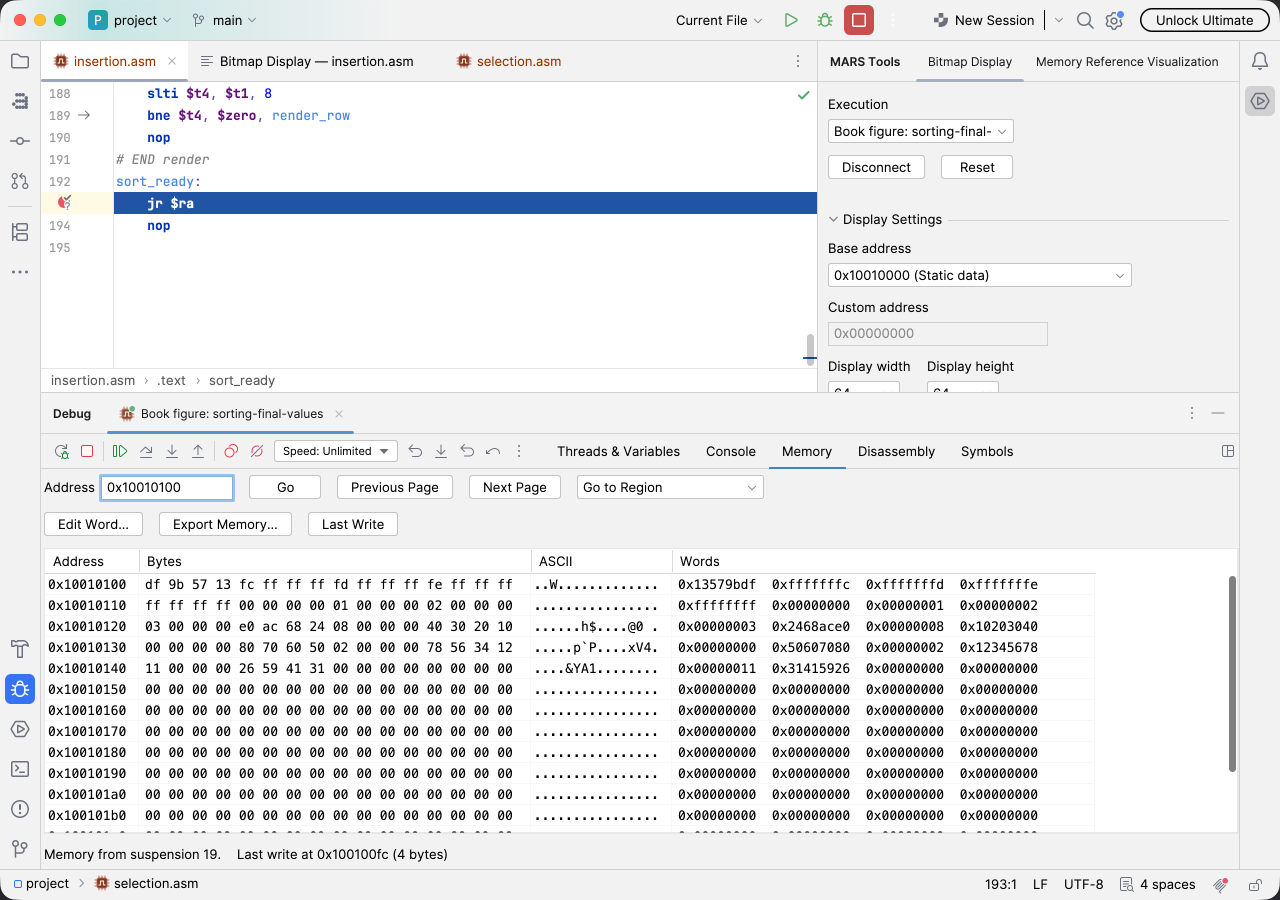
\includegraphics[width=0.78\linewidth,artifact,trim={\MARSfinalstateLeft{} \MARSfinalstateBottom{} \MARSfinalstateRight{} \MARSfinalstateTop{}},clip]{packages/009-sorting-visualizer/captures/f04-final/values.png}};
    \begin{scope}[shift={(state.south west)},x={($(state.south east)-(state.south west)$)},y={($(state.north west)-(state.south west)$)}]
      \draw[black,line width=0.7pt] (0.191919192,0.043010753) rectangle (0.983838384,0.720430108);
      \node[draw=black,fill=white,circle,inner sep=1.5pt,font=\footnotesize] at ($(0.191919192,0.720430108)+(-3mm,0)$) {2};
    \end{scope}
    \node[anchor=north west,inner sep=0,font=\small\bfseries] (memory-title) at ([yshift=-1mm]state.south west) {Algorithm, phase and completed-exchange count};
    \node[anchor=north west,inner sep=0] (memory) at ([yshift=-1mm]memory-title.south west) {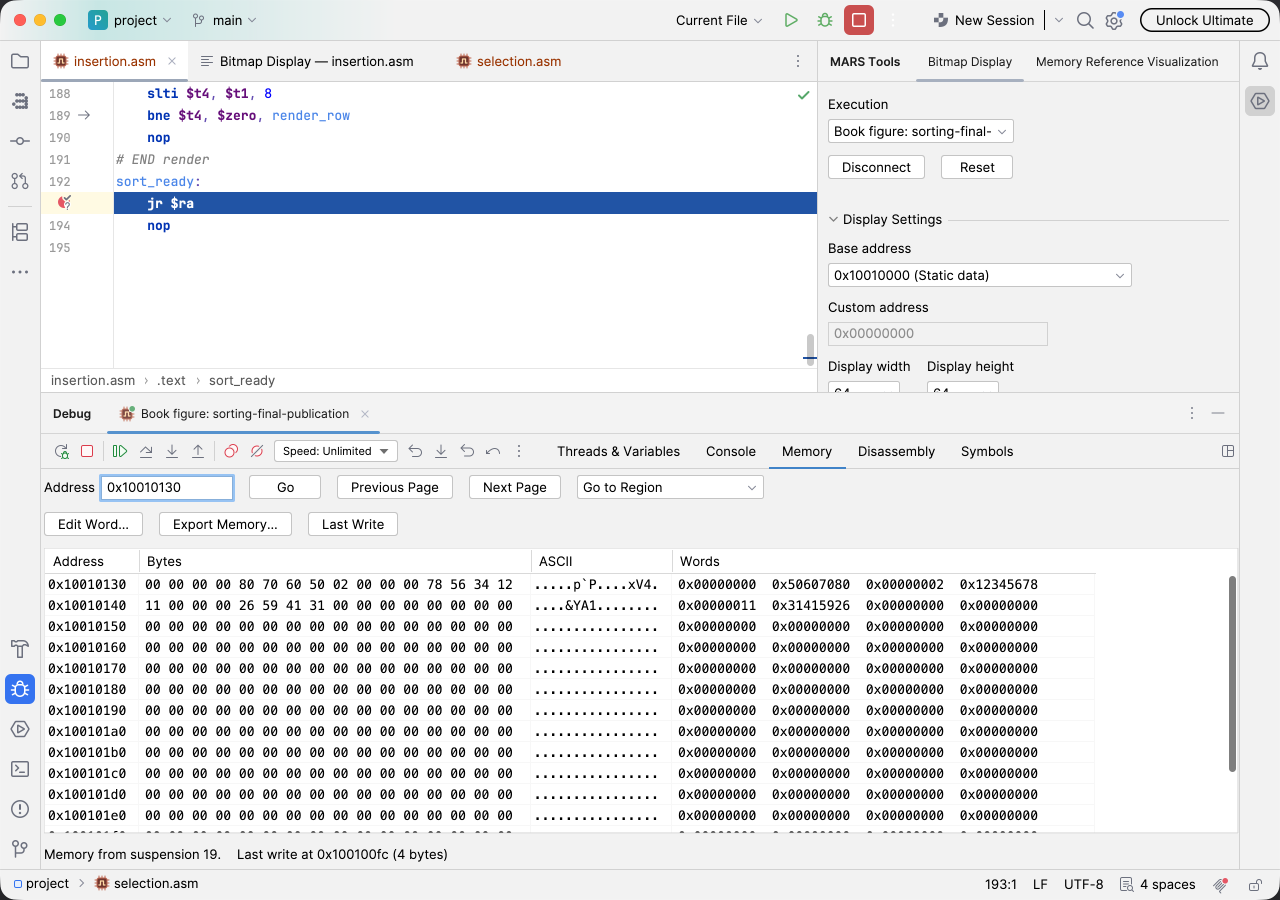
\includegraphics[width=0.78\linewidth,artifact,trim={\MARSfinalmemoryLeft{} \MARSfinalmemoryBottom{} \MARSfinalmemoryRight{} \MARSfinalmemoryTop{}},clip]{packages/009-sorting-visualizer/captures/f04-final/publication.png}};
    \begin{scope}[shift={(memory.south west)},x={($(memory.south east)-(memory.south west)$)},y={($(memory.north west)-(memory.south west)$)}]
      \draw[black,line width=0.7pt] (0.191919192,0.055555556) rectangle (0.983838384,0.638888889);
      \node[draw=black,fill=white,circle,inner sep=1.5pt,font=\footnotesize] at ($(0.191919192,0.638888889)+(-3mm,0)$) {3};
    \end{scope}
    \node[anchor=north west,inner sep=0,font=\small\bfseries] (plot-title) at ([yshift=-1mm]memory.south west) {Complete published framebuffer};
    \node[anchor=north west,inner sep=0] (plot) at ([yshift=-1mm]plot-title.south west) {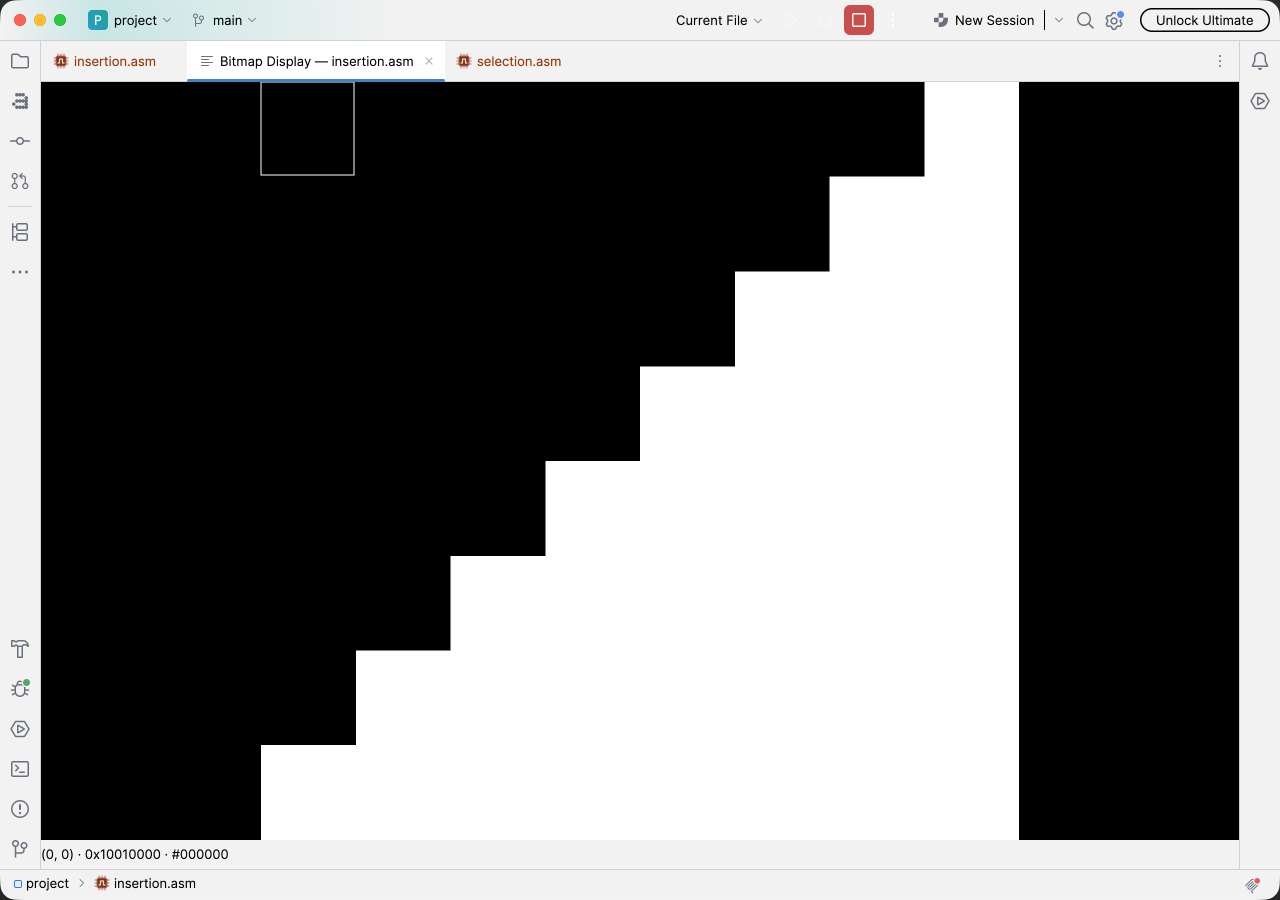
\includegraphics[width=0.24\linewidth,artifact,trim={\MARSfinalplotLeft{} \MARSfinalplotBottom{} \MARSfinalplotRight{} \MARSfinalplotTop{}},clip]{packages/009-sorting-visualizer/captures/f04-final/bitmap.png}};
    \begin{scope}[shift={(plot.south west)},x={($(plot.south east)-(plot.south west)$)},y={($(plot.north west)-(plot.south west)$)}]
      \draw[black,line width=0.7pt] (0.000000000,0.000000000) rectangle (1.000000000,1.000000000);
      \node[draw=black,fill=white,circle,inner sep=1.5pt,font=\footnotesize] at ($(0.000000000,1.000000000)+(-3mm,0)$) {4};
      \foreach \c in {0,...,7} {\node[anchor=north,font=\scriptsize,inner sep=0] at ({(\c+0.5)/8},-0.035) {\c}; \node[anchor=east,font=\scriptsize,inner sep=0] at (-0.025,{1-(\c+0.5)/8}) {\c};}
      \node[anchor=north,font=\scriptsize,inner sep=0] at (0.5,-0.11) {$x$}; \node[anchor=east,font=\scriptsize,inner sep=0] at (-0.10,0.5) {$y$};
    \end{scope}
  \end{tikzpicture}
  \par\smallskip
  \begin{minipage}{\linewidth}
    \small
    \begin{enumerate}
      \item The condition \texttt{\$s2 == 8} selects the final renderer call after the outer loop has finished. It distinguishes this pause from the preceding seventeenth-exchange frame. The blue return will lead to \texttt{done}, where the caller selects the normal exit service.
      \item The array is $[-4,-3,-2,-1,0,1,2,3]$ in signed ascending order. Sorting preserved the original multiset. Its first and last words are \texttt{0xfffffffc} and \texttt{0x00000003}; a hexadecimal display does not by itself imply unsigned ordering.
      \item Phase 2 marks completion. The bytes \texttt{11 00 00 00} at \texttt{0x10010140} encode hexadecimal \texttt{0x11}, or decimal 17 completed exchanges. The final publication changes phase and redraws the array without incrementing that count. This is insertion\textquotesingle s result; the selection run takes five exchanges on the same input.
      \item Heights increase from one to eight, and their first white rows decrease from 7 to 0. The entire last row is white. The same image was already present after insertion\textquotesingle s last exchange; phase 2 and the final-call condition distinguish completion from that earlier publication.
    \end{enumerate}
  \end{minipage}
  \caption{Insertion sort publishes its ascending array after seventeen exchanges.}
  \label{capture:009-sorting-visualizer-f04-final}
\end{figure}
\par
